\section{Results and Discussion}

Response times and accuracy was considered for analysis. Accuracy was calculated as the ratio of estimated to actual reach. Estimated maximum reach was determined by the crossover point from yes to no responses. (Fig. \ref{fig:cross_over}) The actual reach was measured after the experiment. A crossover point greater than 1 means over estimation, a crossover point smaller than 1 means under estimation. 

\begin{figure}
\centering
  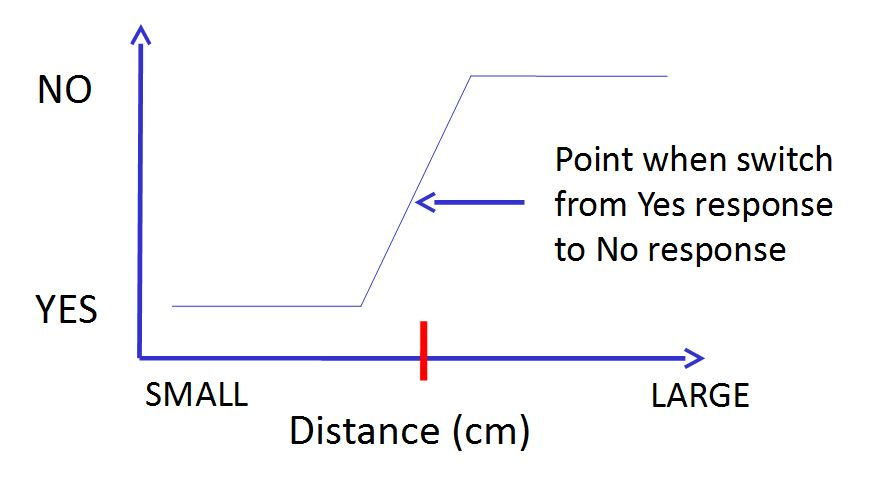
\includegraphics[width=0.75\textwidth]{cross_over}
  \caption{Crossover point: ratio of estimated reach to actual reach.} 
  \label{fig:cross_over}
\end{figure}

\subsection{Response Time}

Firstly, response time did not significantly increase with a greater rotation of the chair. This is not inline with our hypothesis that participants show different reaction times for different locations around the table. Therefore we conclude that there is no cost in reaction time because of “mental rotation of the self in 3D”. An explanation for the consistent reaction times for different rotations could be a visual heuristic used by participants. It is possible that participants imagine a circle on the table which indicates how far they assume they are able to reach. This would make it unnecessary to actively rotate oneself to the target location so that reaction times are independent from the angle of the rotation.

Secondly, as shown in Fig. \ref{fig:no_arm_responst_time_dist} response times in the no arm condition were overall higher than in the shorter/longer arm condition. Since the no arm condition was always the first of the two trial phases this result could be caused by a training effect. Participants were less experienced with the task and therefore required more time to respond. Furthermore they have not yet had any control over their virtual arm so that their judgment is solely based on their imagination.  After having controlled their virtual arm in the adaptation phase, participants get a better understanding of how far they can reach in the second trial phase. This could also cause shorter reaction times in the second trial phase (shorter or longer arm condition).

\begin{figure}
\centering
  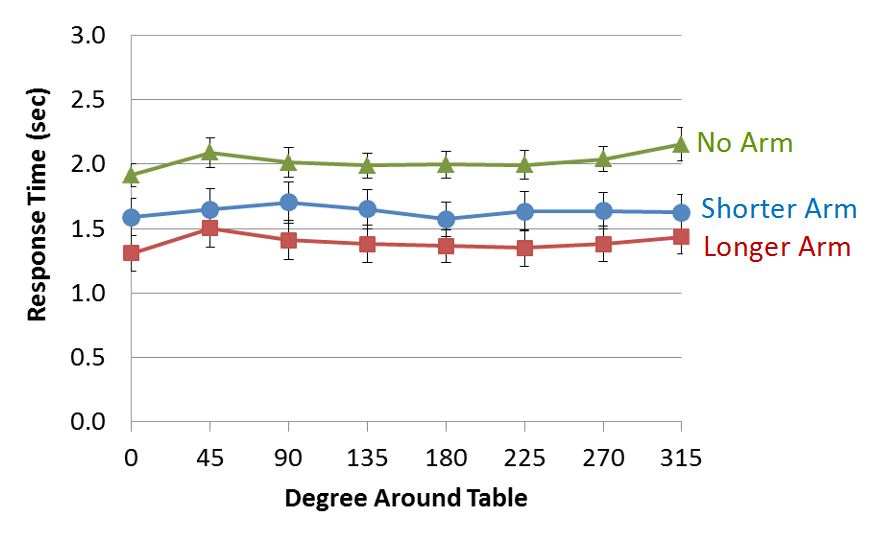
\includegraphics[width=0.75\textwidth]{all_response_time}
  \caption{Response times of different chair angles around the table in all conditions} 
  \label{fig:all_response_time}
\end{figure}

For each condition there is a clear peak of response times in relation to a specific distance of the ball from the edge of the table. The overall shape of the graph can be described as an upside down 'v' and therefore showing lower response times the shorter and higher distances get. In the no arm condition the peak is at 45 cm from the edge of the table with a response time of 2.5 seconds. (Fig \ref{fig:no_arm_responst_time_dist}) The peak response times in this graph indicate that it was the most difficult to make a judgment at a certain distance from the edge of the table. We assume that this distance must be very close to the participant's estimated maximum reaching distance. The closer the ball is to the participant's maximum reaching distance the more difficult it is to make a decision, because a yes and no response become equally likely.
Looking at shorter and higher distances one can observe the opposite effect of lower response times. Since it is obvious that an object can be reached when it is very near (or can not be reached when it is very far) it also easier to make a decision which results in lower response times. 

In the shorter arm condition the peak is at 30 cm from the edge of the table with a response time of 2.1 seconds. And in the longer arm condition the peak is at 40 cm with a response time of 1.7 seconds. (Fig \ref{fig:short_long_arm_responst_time_dist}) Expectedly, in the shorter arm condition participants show a peak reaction time at a shorter distance of the ball from the edge of the table than in the longer arm condition. Thus, having perceived and controlled their virtual arm not only results in shorter reaction times. It also affects the estimated maximum reaching distance. Having Perceived and controlled a shorter arm causes participants to experience a shorter maximum reaching distance and vise versa. 

Comparing the distances of shorter/longer arm condition at peak reaction times (30cm and 40cm) with the no arm condition it is interesting to observe that both the distances of shorter and longer arm condition are smaller than in the no arm condition (45cm). Without the data provided in the experiment one would probably assume that the distances must be higher for the the longer arm condition and smaller for the shorter arm condition. A general explanation for this effect might be the fact that participants are inclined to overestimate their maximum reaching distance without having perceived and controlled the virtual arm. Even if participants were told they should make a decision based on the fact that they can not lean forward, we assume they still incorporate such an increase in range of motion in their judgments, which leads to the overestimation. The opposite effect occurs after having experienced they virtual arm, because they have now experienced that their virtual arm will not reach further when they lean forward. That is because the virtual arm has a fixed shoulder position which is calculated according to the participant's actual bodily dimensions. Virtual arm movements are only animated and deducted by the controller movements (controllers attached to participants wrists). Also having perceived and controlled the virtual arm allows participants to get a visual ruler and therefore a more realistic perception of how far they are able to reach. Both the acceptance that they can not lean forward and the visual ruler provided in the adaptation phase are possible explanations for the decreased estimated maximum reaching distances in both the shorter and longer arm conditions.

Comparing the peak reaction times in the shorter and longer arm condition (1.7 seconds vs. 2.1 seconds) the peak reaction times in the shorter arm condition are significantly higher than in the longer arm condition. We assume that experiencing a shorter arm makes participants feel less comfortable and confident about decisions even if they do not know that the arm was shorter. Those assumptions needed to be verified with confidential votes in possible future replications or follow-up studies.

\begin{figure}
\centering
  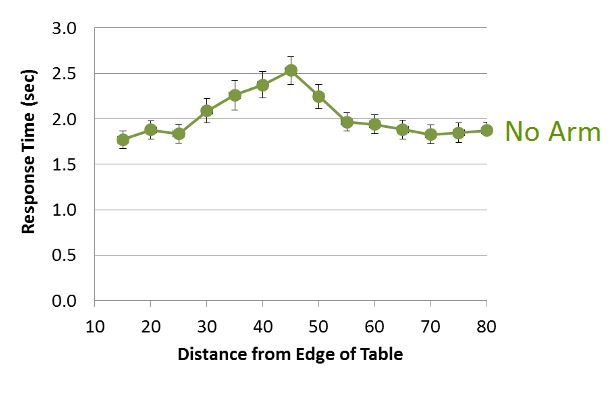
\includegraphics[width=0.75\textwidth]{no_arm_responst_time_dist}
  \caption{Response times in relation to the edge of the table in the no arm condition.} 
  \label{fig:no_arm_responst_time_dist}
\end{figure}

\begin{figure}
\centering
  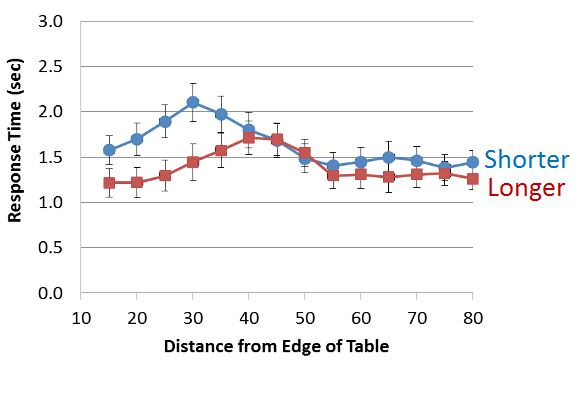
\includegraphics[width=0.75\textwidth]{short_long_arm_responst_time_dist}
  \caption{Response times in relation to the edge of the table in the shorter/longer arm condition.} 
  \label{fig:short_long_arm_responst_time_dist}
\end{figure}

\subsection{Accuracy}

In the no arm condition accuracy (crossover point) ranged from 1.15 to 0.9 . The highest estimation was at 0 degrees. The lowest estimation was at 135 degrees. (Fig. \ref{fig:no_arm_co})

\begin{figure}
\centering
  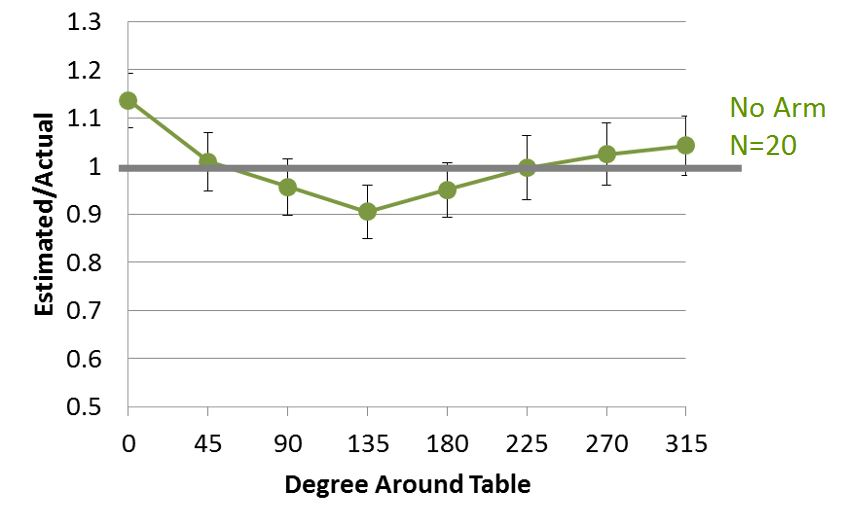
\includegraphics[width=0.75\textwidth]{no_arm_co}
  \caption{Accuracy (crossover point) of different chair angles around the table in the no arm condition} 
  \label{fig:no_arm_co}
\end{figure}

 In the shorter arm condition accuracy (crossover point) ranged from 1.1 to 0.85. The highest estimation was at 0 degrees. The lowest estimation was at 90 degrees. In the longer arm condition accuracy (crossover point) ranged from 0.66 to 0.82 . The highest estimation was at 0 degrees. The lowest estimation was at 135 degrees. (\ref{fig:short_long_arm_co}) 
 
 In all conditions the lowest estimations were between 90 to 135 degrees. This means most low estimations have occured for trials in which the ball was on the left half of the rounds table (degrees were defined clockwise around the table with 0 degrees at the participant's actual location). Since all participants were right-handed their judgments may have been less confident for trials in which the ball was in the left half of the table. 
 
 An general interaction between degree around the table and accuracy could only be found for 0 degrees, because in all conditions the estimation at 0 degrees are the highest. This is probably due to the fact that confidence is higher in the first person perspective. No significant effect could be found for the opposite position at 180 degrees. Also for all other degrees there was no significant interaction because such effects need to occur pairwise (45/215, 90/270, 135/225) which was not the case.
 
 Participants in both the shorter and longer arm condition show overall lower estimations than in the now arm condition, which is inline with the observation of reaction times. 
 

 
 \begin{figure}
\centering
  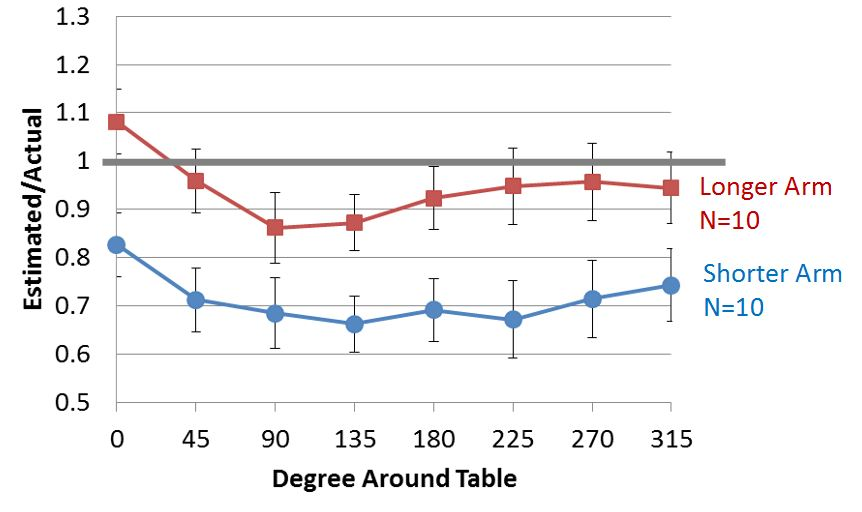
\includegraphics[width=0.75\textwidth]{short_long_arm_co}
  \caption{Accuracy (crossover point) of different chair angles around the table in the shorter/longer arm condition} 
  \label{fig:short_long_arm_co}
\end{figure}

\newpage